\chapter{Métodos de Simulación de Monte-Carlo} \label{Capitulo 3}

Este capítulo se centra en la introducción de varios métodos de integración sobre una función de probabilidad combinando la integración de Monte Carlo con alguna técnica de simulación estocástica. Además, se presentarán otros dos grupos de métodos de este tipo para la generación de muestras que, junto con lo anterior,  permiten calcular el valor de integrales sobre funciones de probabilidad.\cite{pajares2010aprendizaje}

\section{Integración de Monte-Carlo}
Para estudiar este método en profundidad, utilizaremos la siguiente notación:
$U$ representa una variable aleatoria y $\cjtoVarAl$ un conjunto de ellas, y en minúscula, $u$, $\unCjtoVarAl$, para valores específicos, respectivamente. $\todasVar$ será el conjunto de todas las variables del problema, siendo $X$, $x$, $\varOculBfMay$, $\varOculBfMin$, las variables ocultas (desconocidas) e $\textit{Y}$, $y$, $\varObsBfMay$, $\varObsBfMin$, las observadas (medidas). Para las variables de un conjunto, se usará un subíndice $\left(U_g \in \cjtoVarAl\right)$, y para un subconjunto de variables indexadas desde $k$ hasta $s$ usaremos un subíndice \textit{k:s}. Para el $i$-ésimo valor de una muestra se indicará con el superíndice ($i$) y para su peso, $w(\cdot)$.

En cuanto a funciones, la densidad de probabilidad original sobre la que se desea integrar será $p(\cdot)$, mientras que $f(\cdot)$ será una función genérica. Además, una densidad de probabilidad genérica será $Pr(\cdot)$, la densidad auxiliar para obtener las muestras se denotará $q(\cdot)$, la operación de muestreo respecto a una densidad $s\left(\cjtoVarAl\right)$ como $\unCjtoVarAli \thicksim s\left(\cjtoVarAl\right)$  y, finalmente, la función delta de Dirac, $\delta\left(\cdot\right)$.

Esta técnica consigue aproximar el resultado de la integral \ref{ec:3.1}, cuyo valor corresponde con el esperado de una serie de funciones, útil para la resolución de problemas de aprendizaje, cuyo cálculo exacto se reduce a un conjunto muy específico de funciones.
\begin{equation}
    I = E_{p\left(\cjtoVarAl\right)} \left[f\left(\cjtoVarAl\right)\right] = \int f\left(\cjtoVarAl\right)p\left(\cjtoVarAl\right)d\cjtoVarAl 
    \label{ec:3.1}
\end{equation}
La técnica de integración de  Monte-Carlo evalúa $f\left(\textbf{\textit{U}}\right)$ sobre un conjunto $\left\{ \textbf{\textit{u}}^{(1)}, \textbf{\textit{u}}^{(2)}, \dots, \textbf{\textit{u}}^{(N)} \right\}$ distribuidas según $p\left(\textbf{\textit{U}}\right)$.

El método de integración, pues, aproxima \ref{ec:3.1} por medio de la siguiente expresión:
\begin{equation}
    I_{N} = \frac{1}{N} \sum_{i=1}^{N} f\left(\textbf{\textit{u}}^{(i)}\right) \quad con \quad \textbf{\textit{u}}^{(i)} \thicksim p\left(\textbf{\textit{U}}\right) \label{ec:3.2}
\end{equation}
lo que permite evaluar $f\left(\cjtoVarAl\right)$ en puntos de \cjtoVarAl\, donde la probabilidad no sea nula. Esto se consigue mediante la aproximación de la función original $p\left(\cjtoVarAl\right)$  como sigue:
\begin{equation}
    p_{N}\left(\cjtoVarAl\right) = \frac{1}{N}\sum_{i=1}^{N}\delta\left(\cjtoVarAl - \unCjtoVarAl^{(i)}\right) \quad con \quad \unCjtoVarAl^{(i)} \thicksim p\left(\cjtoVarAl\right)
    \label{ec:3.3}
\end{equation}
Sustituyendo en \ref{ec:3.1} $p\left(\textbf{\textit{U}}\right)$ por $p_{N}\left(\textbf{\textit{U}}\right)$  para comprobar la veracidad de la aproximación:
\begin{equation*}
\begin{split}
    I = \int f\left(\cjtoVarAl\right)p\left(\cjtoVarAl\right)d\cjtoVarAl \simeq
        \int f\left(\cjtoVarAl\right)p_{N}\left(\cjtoVarAl\right)d\cjtoVarAl = \\
        = \frac{1}{N}\sum_{i=1}^{N} \int f\left(\cjtoVarAl\right)\delta\left(\cjtoVarAl - \unCjtoVarAl^{(i)}\right)d\cjtoVarAl = \frac{1}{N}\sum_{i=1}^{N}f\left({\unCjtoVarAl^{(i)}}\right) = I_{N}
\end{split}
\end{equation*}

A través de la ley fuerte de los grandes números se puede comprobar que, si $N \rightarrow \infty$, entonces converge casi seguro $I_{N}\xrightarrow{c.s.}I$. También que, para ciertos pares de funciones $f\left(\cjtoVarAl\right)$, $p\left(\cjtoVarAl\right)$, la varianza de $I_{N}$ decrece  según aumenta $N$.

\section{Simulación estocástica}
La simulación estocástica es el mecanismo responsable de generar el conjunto de muestras y, según sea su naturaleza, distinguir unos métodos de simulación de Monte-Carlo de otros.

\section{Técnicas de generación de muestras}
Las siguientes técnicas forman parte de un amplio conjunto de métodos de muestreo auxiliar. Será clave la noción de \textit{soporte} de una función $p\left(\cjtoVarAl\right)$, que se define como una región o un conjunto de ellas donde sucede $p\left(\cjtoVarAl\right) > 0$. Generalmente, es necesario poder evaluar dicha función o, al menos, un múltiplo de ella, pues en muchas ocasiones se trabajará con la proporción de dos evaluaciones de la función de densidad, por lo que la constante se cancela.

\subsection{Muestreo por rechazo}
El muestreo por rechazo (\textit{Rejection Sampling, RS}) genera un conjunto de muestras distribuidas según la función de densidad de probabilidad original $p\left(\cjtoVarAl\right)$ a través de:
\begin{enumerate}
    \item Una función de densidad auxiliar $q\left(\cjtoVarAl\right)$ para generar los candidatos $\unCjtoVarAl^{(i)}$.
    \item Una función de probabilidad uniforme $\mathcal{U}_{(0,1)}\left(A\right)$ para decidir si los candidatos $\unCjtoVarAl^{(i)}$ son aceptados con una probabilidad proporcional a la diferencia de $p\left(\unCjtoVarAl^{(i)}\right)$ y $q\left(\unCjtoVarAl^{(i)}\right)$.
\end{enumerate}

La función auxiliar debe satisfacer $Mq\left(\cjtoVarAl\right) - p\left(\cjtoVarAl\right) > 0$, con $0 < M < \infty$, lo que fuerza a que tenga el mismo soporte que la original, envolviéndola y, además, haciendo que $\dfrac{p\left(\cjtoVarAl\right)}{Mq\left(\cjtoVarAl\right)} \leq 1$. Así, $\unCjtoVarAl^{(i)} \thicksim q\left(\cjtoVarAl\right)$ es aceptado si $a^{(i)}Mq\left(\unCjtoVarAl^{(i)}\right) < p\left(\unCjtoVarAl^{(i)}\right)$. En otro caso se rechaza y los valores de $\unCjtoVarAl^{(i)}$ y de $a^{(i)}$ se reemplazan por otro par.

\begin{figure}[ht]
    \centering
    \begin{tcolorbox}[colframe=black, colback=white, boxrule=0.5pt, width=0.58\textwidth, sharp corners]
        \begin{minipage}[t]{\linewidth}
        \text{1.} \quad $i=1$ \\
        \text{2.} \quad while $(i \leq N)$ \\ [0.5em]
        \text{3.} \quad \hspace{1em} $\unCjtoVarAli \sim q(\cjtoVarAl)$, \quad $a^{(i)} \sim \mathcal{U}_{(0,1)}\left(A\right)$ \\[0.5em]
        \text{4.} \quad \hspace{1em} if $a^{(i)}Mq(\unCjtoVarAli)< p(\unCjtoVarAli)$ then $i = i + 1$
        \end{minipage}
    \end{tcolorbox}
    \caption{Método de muestreo por rechazo.}
    \label{fig:3.1}
\end{figure}



Esta aceptación y rechazo sucede con una probabilidad $Pr\left(A|\unCjtoVarAl^{(i)}\right) = p\left(\unCjtoVarAl^{(i)}\right) / Mq\left(\unCjtoVarAl^{(i)}\right)$ y de $1-Pr\left(A|\unCjtoVarAl^{(i)}\right)$, respectivamente. Por tanto, cuanto más cercanos sean $p\left(\cjtoVarAl\right)$ y $Mq\left(\cjtoVarAl\right)$ en el soporte de $p\left(\cjtoVarAl\right)$ más eficiente será el método. Es conveniente elegir $q\left(\cjtoVarAl\right)$ de modo que permita fijar valores pequeños de $M$, pues $Pr\left(A\right) = \int Pr\left(A|\cjtoVarAl\right)q\left(\cjtoVarAl\right)d\cjtoVarAl = \dfrac{1}{M} \displaystyle \int p\left(\cjtoVarAl\right)d\left(\cjtoVarAl\right) = \frac{1}{M}$.

También se da que $Pr\left(\cjtoVarAl|A\right) = \dfrac{Pr\left(A|\cjtoVarAl\right)q\left(\cjtoVarAl\right)}{Pr\left(A\right)} = \dfrac{p\left(\cjtoVarAl\right)q\left(\cjtoVarAl\right)M}{Mq\left(\cjtoVarAl\right)} = p\left(\cjtoVarAl\right)$, luego $\unCjtoVarAl^{(i)}$ se distribuyen según la función $p\left(\cjtoVarAl\right)$ original.

Cabe destacar que el método de muestreo por rechazo es igualmente válido si se conoce una expresión de la forma $Cte\cdot p\left(\cjtoVarAl\right)$. Sin embargo, no es sencillo de implementar en problemas multidimensionales complejos, pues es difícil encontrar $q\left(\cjtoVarAl\right)$ y $M$ adecuados para generar pocos rechazos, problema solventable haciendo uso de la versión adaptativa de este mismo método.

\subsection{Muestreo enfatizado} \label{subsec:IS}
En el muestreo enfatizado (\textit{Importance Sampling, IS}), las muestras $\unCjtoVarAl^{(i)}$ se toman de una función de densidad auxiliar  $q\left(\cjtoVarAl\right)$ con soporte igual o mayor que el de $p\left(\cjtoVarAl\right)$. Los pesos $\unPeso$ representan la proporción de la muestra dentro de $p\left(\cjtoVarAl\right)$, midiendo la disonancia entre la densidad original y la auxiliar, es decir, lo lejos que están de ser iguales. Por tanto, al tener que $\unPeso \propto \dfrac{p\left(\unCjtoVarAl^{(i)}\right)}{q\left(\unCjtoVarAl^{(i)}\right)}$, es suficiente con conocer una expresión proporcional a la densidad original $Cte\cdot p\left(\cjtoVarAl\right)$. En este caso, $p\left(\cjtoVarAl\right)$ e $I$ de la ecuación \ref{ec:3.1} se aproximan, respectivamente, como:
\begin{equation}
\begin{aligned}
    &p_{IS} = \sum_{i=1}^{N}\unPeso\delta\left(\cjtoVarAl - \unCjtoVarAl^{(i)}\right);
    \quad I_{IS} = \sum_{i=1}^{N}\unPeso f\left(\unCjtoVarAl^{(i)}\right) \\
    &\text{con} \quad \unCjtoVarAl^{(i)} \thicksim q\left(\cjtoVarAl\right), \quad \unPeso \propto \frac{p\left(\unCjtoVarAl^{(i)}\right)}{q\left(\unCjtoVarAl^{(i)}\right)}, \quad \sum_{i=1}^{N} \unPeso = 1
\end{aligned}
\label{ec:3.4}
\end{equation}

El pseudocódigo de la Figura \ref{fig:3.2} recoge el algoritmo para la generación de $N$ muestras $\unCjtoVarAli$ con sus correspondientes pesos $\unPeso$.

\begin{figure}[ht]
    \centering
    \begin{tcolorbox}[colframe=black, colback=white, boxrule=0.5pt, width=0.81\textwidth, sharp corners]
        \begin{minipage}[t]{\linewidth}
            \text{1.} \quad $T = 0$ \\
            \text{2.} \quad for $(i=1:N)$ \\
            \text{3.} \quad \hspace{1em} $\unCjtoVarAli \sim q(\cjtoVarAl)$, \quad $\unPeso=\dfrac{p\left(\unCjtoVarAl^{(i)}\right)}{q\left(\unCjtoVarAl^{(i)}\right)}$, \quad $T = T + \unPeso$ \\[0.5em]
            \text{4.} \quad for $(i=1:N)$ \\[0.5em]
            \text{5.} \quad \hspace{1em} $\unPeso = \dfrac{\unPeso}{T}$
        \end{minipage}
    \end{tcolorbox}
    \caption{Método genérico de muestreo enfatizado.}
    \label{fig:3.2}
\end{figure}

Las ecuaciones de \ref{ec:3.4} se derivan de la expresión \ref{ec:3.1} introduciendo la función de muestreo auxiliar $q\left(\cjtoVarAl\right)$. Además, se considera que la función de muestreo $w\left(\cjtoVarAl\right)q\left(\cjtoVarAl\right)$ puede aproximarse mediante $p_{IS}\left(\cjtoVarAl\right)$ combinando las probabilidades de densidad puntual $\delta\left(\cjtoVarAl-\unCjtoVarAli\right)$ centradas en las $N$ muestras $\unCjtoVarAli$ obtenidas de manera independiente con la función auxiliar $q\left(\cjtoVarAl\right)$ y pesadas según $w\left(\unCjtoVarAli\right)$:

\begin{equation*}
    \begin{aligned}
        I &= \int f\left(\cjtoVarAl\right)p\left(\cjtoVarAl\right)d\cjtoVarAl = \int f\left(\cjtoVarAl\right)\dfrac{p\left(\cjtoVarAl\right)}{q\left(\cjtoVarAl\right)}q\left(\cjtoVarAl\right)d\cjtoVarAl = \int f\left(\cjtoVarAl\right)w\left(\cjtoVarAl\right)q\left(\cjtoVarAl\right)d\cjtoVarAl \simeq  \\
        &\simeq \int f\left(\cjtoVarAl\right)w\left(\cjtoVarAl\right)\dfrac{1}{N}\sum_{i=1}^{N}\delta\left(\cjtoVarAl-\unCjtoVarAli\right)d\cjtoVarAl = \int f\left(\cjtoVarAl\right)\dfrac{1}{N}\sum_{i=1}^{N}w\left(\unCjtoVarAli\right)\delta\left(\cjtoVarAl-\unCjtoVarAli\right)d\cjtoVarAl
    \end{aligned}
\end{equation*}

La elección de $q\left(\cjtoVarAl\right)$ hace controlar la región de donde se obtienen las muestras, y así introducir cualquier tipo de conocimiento previo que se tenga de la original $p\left(\cjtoVarAl\right)$. Además, como se quiere aproximar el valor integral, es conveniente minimizar la varianza. Para ello, la función auxiliar óptima es $q^*\left(\cjtoVarAl\right) = \dfrac{\abs{f\left(\cjtoVarAl\right)}p\left(\cjtoVarAl\right)}{\int \abs{f\left(\cjtoVarAl\right)}p\left(\cjtoVarAl\right)}$, cuyo valor minimiza la varianza $E_{q\left(\cjtoVarAl\right)}\big[w^2\left(\cjtoVarAl\right) f^2\left(\cjtoVarAl\right)\big]$ (si $E_{q\left[\cjtoVarAl\right)}\left[x\right]$ denota la esperanza, $E_{q\left(\cjtoVarAl\right)}\left[x^2\right]$ denota la varianza) \cite{pajares2010aprendizaje}. De ella no se puede muestrear directamente, pero nos señala que se pierde eficiencia si el numerador se anula. Si se quiere obtener los valores integrales para varias funciones generales $f\left(\cjtoVarAl\right)$, se puede emplear varias o una sola $q\left(\cjtoVarAl\right)$, que ignore las funciones generales e intente aproximarse a $p\left(\cjtoVarAl\right)$.

Sin embargo, la elección de una función auxiliar eficiente es más complicado en el caso multidimensional. Existen técnicas para sortear este inconveniente, como el muestreo por importancia adaptativo o el muestreo enfatizado secuencial (\textit{Sequential Importance
Sampling, SIS}), implementado en los filtros de partículas.

\subsection{Remuestreo por pesos}\label{subsec:WR}
En el método de remuestreo por pesos (\textit{Weighted Resampling, WR}) se aproxima una función de densidad $p_{A}\left(\cjtoVarAl\right)$, que es una combinación de $N_{A}$ funciones de densidad puntuales $\delta\left(\cjtoVarAl-\unCjtoVarAl_{A}^{(i)}\right)$, centradas en $\unCjtoVarAlA$ y ponderadas según $\unPesoA$, por otra función $p_{B}\left(\cjtoVarAl\right)$ de la misma clase.

Los centros de $p_{B}\left(\cjtoVarAl\right)$ son muestreados entre los valores de $\unCjtoVarAlA$ mediante $r\left(\cjtoVarAl\right)$, la cual indica en qué regiones del espacio generar una determinada cantidad de muestras, y la función de probabilidad $q\left(I|\unCjtoVarAl_{A}^{(i)}\right)$, que elige las muestras de forma proporcional a su correspondiente valor $r\left(\unCjtoVarAl_{A}^{(i)}\right)$. Los pesos $\unPesoB$ son el cociente de los pesos en la densidad original $\unPesoA$ entre el valor $r\left(\unCjtoVarAlA\right)$, el cual toman de la función de remuestreo $\left(\unCjtoVarAlB= \unCjtoVarAlA\right)$:

\begin{equation}
\begin{aligned}
    p_{A}\left(\cjtoVarAl\right) &= \sum_{i=1}^{N_{A}}\unPesoA\delta\left(\cjtoVarAl-\unCjtoVarAlA\right); \quad
    p_{B}\left(\cjtoVarAl\right) = \sum_{i=1}^{N_{B}}\unPesoB\delta\left(\cjtoVarAl-\unCjtoVarAlB\right) \\
    &\text{con} \quad \unCjtoVarAlA = \unCjtoVarAlB, \quad i \thicksim q\left(I|\unCjtoVarAl_{A}^{(i)}\right), \quad q\left(I|\unCjtoVarAl_{A}^{(i)}\right) \propto r\left(\unCjtoVarAl_{A}^{(i)}\right) \\
    &\textit{w}\left(\unCjtoVarAl_{B}^{\left(j\right)}\right) \propto \frac{\unPesoA}{r\left(\unCjtoVarAl_{A}^{(i)}\right)}, \quad \sum_{i=1}^{N_{B}}\textit{w}\left(\unCjtoVarAl_{B}^{\left(j\right)}\right) = 1
\end{aligned}
\label{ec:3.5}
\end{equation}

El pseudocódigo de la Figura \ref{fig:3.3} ilustra la generación de $N$ muestras $\unPesoB$ con sus correspondientes pesos $\unPesoB$.

\begin{figure}[h]
    \centering
    \begin{tcolorbox}[colframe=black, colback=white, boxrule=0.5pt, width=0.8\textwidth, sharp corners]
        \parbox[t]{\linewidth}{1. \quad $T = 0$} \\
        \parbox[t]{\linewidth}{2. \quad for $(j=1:N)$} \\[0.5em]
        \parbox[t]{\linewidth}{3. \quad \hspace{1em} $I \sim q(I|\unCjtoVarAlA),$} \\[0.5em]
        \parbox[t]{\linewidth}{4. \quad \hspace{1em} $\unCjtoVarAlB = \unCjtoVarAlA$, \quad $\unPesoB = \dfrac{\unPesoA}{r\left(\unCjtoVarAlA\right)}$, \quad $T = T + \unPesoB$} \\[0.5em]
        \parbox[t]{\linewidth}{5. \quad \text{for} $(j=1:N)$ \quad $\unPesoB=\dfrac{\unPesoB}{T}}$
    \end{tcolorbox}
    \caption{Método genérico de remuestreo por pesos.}
    \label{fig:3.3}
\end{figure}

Estas aproximaciones garantizan que, cuando $N \rightarrow \infty$, ambas distribuciones converjan, a condición de que el soporte de $r\left(\cjtoVarAl\right)$ contenga al de $p_{A}\left(\cjtoVarAl\right)$.

Además de elegir la función $r\left(\cjtoVarAl\right)$, cuando se utiliza un método de remuestreo por pesos, es necesario seleccionar el método de muestreo proporcional $q\left(I|\unCjtoVarAl_{A}^{(i)}\right)$, usualmente el muestreo multinomial, el sistemático y el residual, los cuales no trataremos en esta sección \cite{pajares2010aprendizaje}.

La base del método de remuestreo por pesos se asemeja a la empleada por el método de muestreo enfatizado, dado que al incorporar una nueva función de muestreo proporcional a $r\left(\cjtoVarAl\right)$, esta se encuentra en el denominador de la función que determina los pesos $\unPesoB$. La libertad de elección de $r\left(\cjtoVarAl\right)$ nos permite generar muestras en el soporte que merecen ser estudiadas en profundidad. Es habitual elegir el valor de $r\left(\unCjtoVarAlA\right)$ igual al de los pesos $\unPesoA$, con el fin de que las nuevas muestras $\unCjtoVarAlB$ se concentren en las regiones más probables de la función de densidad original, y que $\unPesoB = \dfrac{1}{N}$, lo cual cobra sentido en la creación de algunos filtros de partículas, sobre los que hablaremos en la sección \ref{sec:Filtros de Partículas}.


\section{Métodos de simulación por cadenas de Markov}
El fundamento de método de muestreo mediante cadenas de Markov ($\textit{Markov Chains, MC}$) reside en que la siguiente muestra, $\unCjtoVarAli$, es generada mediante un proceso estocástico definido por una función de probabilidad, \textit{kernel de transición}, $K\left(\cjtoVarAl|\unCjtoVarAliMenos\right)$, la cual sólo depende de la muestra inmediatamente anterior (\textsl{propiedad de Markov}).
Para la aproximación de la función de densidad original, se usarán las $N$ últimas muestras como sigue:

\begin{equation}
    p_{MC} = \frac{1}{N}\sum_{j = B}^{N+B}\delta\left(\cjtoVarAl-\unCjtoVarAlj\right) \quad con \quad \unCjtoVarAlj \thicksim K\left(\unCjtoVarAlj|\unCjtoVarAljMenos\right)
    \label{ec:3.6}
\end{equation}

El pseudocódigo de la Figura \ref{fig:3.4} muestra cómo se generan las $B+N$ muestras, de las cuales se desechan las $B$ primeras.
\begin{figure}[ht]
    \centering
    \begin{tcolorbox}[colframe=black, colback=white, boxrule=0.5pt, width=0.48\textwidth, sharp corners]
        \parbox[t]{\linewidth}{1. \quad $i=1, \quad j=1$, \quad \text{fijar } $\unCjtoVarAl^{(0)}$} \\[0.5em]
        \parbox[t]{\linewidth}{2. \quad while $(i \leq N)$} \\[0.5em]
        \parbox[t]{\linewidth}{3. \quad \hspace{1em} $\unCjtoVarAli \sim K \left( \cjtoVarAl \mid \unCjtoVarAliMenos \right)$} \\[0.5em]
        \parbox[t]{\linewidth}{4. \quad \hspace{1em} if $j \geq B$ \text{then } $i = i + 1$,} \\[0.5em]
        \parbox[t]{\linewidth}{5. \quad \hspace{1em} \text{else } $\unCjtoVarAliMenos = \unCjtoVarAli$, \quad $j = j + 1$}
    \end{tcolorbox}
    \caption{Método genérico de muestreo por cadena de Markov.}
    \label{fig:3.4}
\end{figure}


Para que el proceso definido con el kernel de transición, conocido como cadena de Markov, genere las muestras acorde a la función de probabilidad original $p\left(\cjtoVarAl\right)$, se requiere de:

\begin{enumerate}
    \item La convergencia de la cadena de Markov tras la toma de unas muestras iniciales posteriormente deshechadas.
    \item La función de probabilidad estacionaria a la que converja ha de ser $p\left(\cjtoVarAl\right)$. \label{item:2}
\end{enumerate}

Esto es, que $K\left(\cjtoVarAl|\unCjtoVarAliMenos\right)$ cumpla las condiciones de ser \textsl{irreducible} (visita todo el soporte en tiempo limitado), \textsl{aperiódica} (no fluctuación entre distintas regiones del soporte de forma periódica) y \textsl{recurrente de forma positiva} (para la existencia de función estacionaria).

Una condición suficiente para $\ref{item:2}$ es que la cadena sea reversible y, por tanto, en el momento estacionario la velocidad de la transición sea igual en ambos sentidos:
\begin{equation}
    p\left(\unCjtoVarAliMenos\right)K\left(\unCjtoVarAli|\unCjtoVarAliMenos\right) = p\left(\unCjtoVarAli\right)K\left(\unCjtoVarAliMenos|\unCjtoVarAli\right)
    \label{ec:3.7}
\end{equation}
Una función de probabilidad $p\left(\cjtoVarAl\right)$ puede dar lugar a distintas cadenas de Markov, cada una con una velocidad a priori distinta, lo que hace más beneficioso el uso de unas frente a otras. Al tomar las últimas $N$ muestras, antes de la convergencia, las $B$ primeras se suelen desechar (\textit{burn-in}), luego la aproximación de $p\left(\cjtoVarAl\right)$ se encuentra en el rango entre $B$ y $B+N$. La elección del valor inicial de $\unCjtoVarAl^{(0)}$ influye en el valor del $\textit{burn-in}$, lo que a su vez repercute, además del número necesario de muestras $N$, en el error de la aproximación mediante $p_{MC}$. Por ello, se suelen emplear otras técnicas avanzadas para su obtención. También es posible generar los datos utilizando cadenas independientes y/o utilizar los subconjuntos de muestras obtenidas una vez dada la convergencia. Finalmente, pese a la dificultad de construcción de una cadena $K\left(\cjtoVarAl|\unCjtoVarAliMenos\right)$, existen algunas cadenas generales ya definidas dentro de algunos métodos con un uso amplio plausible.

\subsection{Cadena general para los métodos de Metrópolis-Hastings y Gibbs}\label{CadenaGeneral}
El tipo de cadena elegida para estos procedimientos permite atacar problemas en los que se conoce $Cte\cdot p\left(\cjtoVarAl\right)$ en vez de $p\left(\cjtoVarAl\right)$. La generalidad de $K\left(\cjtoVarAl|\unCjtoVarAliMenos\right)$ recae en la posibilidad de modelar su comportamiento mediante la densidad condicionada $q\left(\cjtoVarAl|\unCjtoVarAliMenos\right)$.

La cadena genera valores para $\unCjtoVarAli$ a partir de la densidad condicionada anterior, con probabilidad de aceptación Pr$\left(A|\cjtoVarAl, \unCjtoVarAliMenos\right)$, e iguales a $\unCjtoVarAliMenos$ con probabilidad de rechazo de Pr$\left(\neg A|\unCjtoVarAliMenos\right)$. La probabilidad de aceptación de Pr$\left(A|\cjtoVarAl, \unCjtoVarAliMenos\right)$ está supeditada a a los valores de $p(\cdot)$, $q(\cdot)$, evaluadas de manera directa e inversa sobre los valores de $\cjtoVarAl = \unCjtoVarAli$ y $\unCjtoVarAliMenos$.

Así, por construcción, se asegura que la cadena $K\left(\cjtoVarAl|\unCjtoVarAliMenos\right)$ sea reversible (\ref{ec:3.7}) y, por tanto, que la función de probabilidad estacionaria sea $p\left(\cjtoVarAl\right)$. Además, forzando que el soporte de $q\left(\cjtoVarAl|\unCjtoVarAliMenos\right)$ incluya el soporte de $p\left(\cjtoVarAl\right)$ se logra la irreductibilidad y la aperiodicidad por la posibilidad de no aceptar la muestra candidata mediante $q\left(\cjtoVarAl|\unCjtoVarAliMenos\right)$. Por tanto, con estas elecciones la cadena $K\left(\cjtoVarAl|\unCjtoVarAliMenos\right)$ consigue generar muestras según $p\left(\cjtoVarAl\right)$.

Dicha cadena se define de la siguiente manera:
\begin{equation}
\begin{aligned}
    K\left(\cjtoVarAl|\unCjtoVarAliMenos\right) &= q\left(\cjtoVarAl|\unCjtoVarAliMenos\right)Pr\left(A|\cjtoVarAl, \unCjtoVarAliMenos\right) +\\
    &\quad + \delta\left(\cjtoVarAl-\unCjtoVarAliMenos\right)Pr\left(\neg A|\unCjtoVarAliMenos\right) \\ \\
    \text{con} \quad \text{Pr}\left(A|\cjtoVarAl, \unCjtoVarAliMenos\right) &= \min\left\{1, \dfrac{p\left(\cjtoVarAl\right)q\left(\unCjtoVarAliMenos|\cjtoVarAl\right)}{p\left(\unCjtoVarAliMenos\right)q\left(\cjtoVarAl|\unCjtoVarAliMenos\right)}\right\} \\
    \text{Pr}\left(\neg A|\unCjtoVarAliMenos\right) = &\int Pr\left(\neg A|\cjtoVarAl, \unCjtoVarAliMenos\right)q\left(\cjtoVarAl|\unCjtoVarAliMenos\right)d\cjtoVarAl \\
    \text{Pr}\left(\neg A|\cjtoVarAl, \unCjtoVarAliMenos\right) &= 1 - \text{Pr}\left(A|\cjtoVarAl, \unCjtoVarAliMenos\right)
\end{aligned}
\label{ec:3.8}
\end{equation}
Al aparecer el cociente $p\left(\cjtoVarAl\right) / p\left(\unCjtoVarAliMenos\right)$, no es necesario conocer la expresión de $p\left(\cjtoVarAl\right)$, por lo que bastaría considerar un múltiplo.

\subsection{Algoritmos de Metropolis-Hastings}
Los algoritmos de esta familia se desarrollan utilizando directamente la cadena de Markov descrita en la sección anterior, implementada en un programa que la emula. El pseudocódigo mostrado en la Figura \ref{fig:3.5} da una posible implementación.

El soporte de la densidad $q\left(\cjtoVarAl|\unCjtoVarAliMenos\right)$ debe incluir al de la original $p\left(\cjtoVarAl\right)$ y la elección de ésta influirá en la velocidad de convergencia del método.

Por un lado, una variante de esta familia de algoritmos es la de Metropolis, en la que la densidad auxiliar se toma simétrica, $q\left(\cjtoVarAl|\unCjtoVarAliMenos\right) = q\left(\unCjtoVarAliMenos|\cjtoVarAl\right)$, quedando entonces $\text{Pr}\left(A|\cjtoVarAl, \unCjtoVarAliMenos\right) = \min\left\{1, \dfrac{p\left(\cjtoVarAl\right)}{p\left(\unCjtoVarAliMenos\right)}\right\}$.

\begin{figure}[ht]
    \centering
    \begin{tcolorbox}[colframe=black, colback=white, boxrule=0.5pt, width=0.8\textwidth, sharp corners]
        \parbox[t]{\linewidth}{1. \quad $i=1, \quad j=1, \quad \text{fijar } \unCjtoVarAl^{(0)}$} \\[0.5em]
        \parbox[t]{\linewidth}{2. \quad while $(i \leq N)$} \\[0.5em]
        \parbox[t]{\linewidth}{3. \quad \hspace{1em} $\unCjtoVarAli \sim  q\left( \cjtoVarAl \mid \unCjtoVarAliMenos \right)$, \quad $a^{(i)} \sim \mathcal{U}_{(0,1)}\left(A\right)$} \\[0.5em]
        \parbox[t]{\linewidth}{4. \quad \hspace{1em} $\text{Pr}\left(A|\unCjtoVarAli, \unCjtoVarAliMenos\right) = \min\left\{1, \dfrac{p\left(\unCjtoVarAli\right)q\left(\unCjtoVarAliMenos|\unCjtoVarAli\right)}{p\left(\unCjtoVarAliMenos\right)q\left(\unCjtoVarAli|\unCjtoVarAliMenos\right)}\right\}$} \\[0.5em]
        \parbox[t]{\linewidth}{5. \quad \hspace{1em} if $a^{(i)} > \text{Pr}\left(A|\unCjtoVarAli, \unCjtoVarAliMenos\right)$ \text{then } $\unCjtoVarAli = \unCjtoVarAliMenos$} \\[0.5em]
        \parbox[t]{\linewidth}{6. \quad \hspace{1em} if $j \geq B$ \text{then } $i = i+1$} \\[0.5em]
        \parbox[t]{\linewidth}{7. \quad \hspace{1em} else $\unCjtoVarAliMenos = \unCjtoVarAli$, \quad $j = j+1$}
    \end{tcolorbox}
    \caption{Algoritmo de Metropolis-Hastings.}
    \label{fig:3.5}
\end{figure}

Por otro lado, la variante conocida como \textsl{muestreador independiente} asume que $q\left(\cjtoVarAl|\unCjtoVarAliMenos\right) = q\left(\cjtoVarAl\right)$, de ahí el nombre, lo que resulta en $\text{Pr}\left(A|\cjtoVarAl, \unCjtoVarAliMenos\right) = \min\left\{1, \dfrac{w\left(\cjtoVarAl\right)}{w\left(\unCjtoVarAliMenos\right)}\right\}$, siendo $w\left(\cjtoVarAl\right) = \dfrac{p\left(\cjtoVarAl\right)}{q\left(\cjtoVarAl\right)}$, función de peso ya presentada en el método IS (\ref{subsec:IS}).
Este método crea una dependencia entre las muestras, de modo que si el peso de una muestra $\unCjtoVarAli$ es mayor que la anterior, se acepta y en caso contrario, se rechaza o se acepta según lo fuerte que sea dicha discrepancia.


\subsection{Método de Gibbs}
El método de simulación de Gibbs, frecuente en problemas multivariables, consiste en una implementación en serie de la cadena de Markov de \ref{CadenaGeneral} y unas funciones de muestreo auxiliar $q(\cdot)$ determinadas. 

Durante el proceso se actualiza cada una de las $U_{g}$ de $\cjtoVarAl = \left\{U_{1}, U_{2}, \dots , U_{G}\right\}$ mediante una cadena distinta $K\left(\cadenaGibbs\right)$, con una probabilidad de aceptación que se rige por la función $p\left(\cadenaGibbs\right)$ y funciones auxiliares $q\left(\cadenaGibbs\right)$. Para cada subíndice $\textit{g}$, $p(\cdot)$ y $q(\cdot)$ coinciden, luego $Pr\left(A|\cjtoVarAl_{k},\unCjtoVarAli_{1:g-1}, \unCjtoVarAliMenos_{g+1:G}\right) = 1$ y, por tanto, el proceso de aceptación del método de Metropolis-Hastings no es necesario, pues se aceptan todas las muestras.

El pseudocódigo que aparece en la Figura \ref{fig:3.6} ilustra las diferentes etapas del método de Gibbs. Cada elemento del bucle interno se relaciona con una de las cadenas muestreadas en serie. El muestreado de $u_k^{(i)}$ de la función $p\left(\cadenaGibbs\right)$ hace que, como se ha comentado antes, desaparezca el proceso de aceptación típico de Metropolis-Hastings.
\begin{figure}[ht]
    \centering
    \begin{tcolorbox}[colframe=black, colback=white, boxrule=0.5pt, width=0.65\textwidth, sharp corners]
        \parbox[t]{\linewidth}{1. \quad $i=1, \quad j=1, \quad \text{fijar } \unCjtoVarAl^{(0)} = \left\{u^{(0)}_{1}, u^{(0)}_{2}, \dots, u^{(0)}_{G}\right\}$} \\[0.5em]
        \parbox[t]{\linewidth}{2. \quad while $(i \leq N)$} \\[0.5em]
        \parbox[t]{\linewidth}{3. \quad \hspace{1em} $g = 1$} \\[0.5em]
        \parbox[t]{\linewidth}{4.\quad \hspace{1em} while ($g \leq G$)} \\[0.5em]
        \parbox[t]{\linewidth}{5.\quad \hspace{2em} $\unCjtoVarAli_g \sim p\left(\cadenaGibbs\right), \quad g = g+1$} \\[0.5em]
        \parbox[t]{\linewidth}{6. \quad \hspace{1em} if $j \geq B$ \text{then } $i = i+1$} \\[0.5em]
        \parbox[t]{\linewidth}{7. \quad \hspace{1em} else $\unCjtoVarAliMenos = \unCjtoVarAli$, \quad $j = j+1$}
    \end{tcolorbox}
    \caption{Método de Gibbs.}
    \label{fig:3.6}
\end{figure}

A la hora de aplicar el método de Gibbs, la dificultad radica principalmente en determinar las funciones de distribución condicional $p\left(\cadenaGibbs\right)$ a partir de la función de probabilidad original $p\left(\cjtoVarAl\right)$. Sin embargo, esto se puede sortear parcialmente si se modela el problema con una \textcolor{red}{red bayesiana. \textbf{(la explico, en anexo...?)}}


\section{Métodos secuenciales de Monte-Carlo}
Los métodos secuenciales de Monte-Carlo, aplicables a problemas multivariables, estos métodos hacen uso de una implementación secuencial del muestreo enfatizado combinado, a elección, con una implementación secuencial del remuestreo por pesos. Por medio de las independencias condicionales de las $U_{g} \in \cjtoVarAl$, generan los $N$ valores $\unCjtoVarAli_{g}$ de $U_{g}$, teniendo en cuenta los valores de $\unCjtoVarAli_{k}$ de las variables $\left\{U_{k}|k \subset \{1:G\right\}\}$ ya muestreadas.

En el diseño del algoritmo interfieren las independencias condicionales propias del problema a resolver y, por tanto, su implementación se adapta a las características específicas de dicho problema. Dado que el método depende del problema, resulta útil escoger un tipo particular de problema para ejemplificar el funcionamiento de esta familia de técnicas. Por ejemplo, para problemas modelables mediante redes bayesianas dinámicas genéricas, un conjunto de métodos secuenciales son los filtros de partículas (\textit{Particle Filters, PF}).

\begin{figure}[ht]
    \centering
    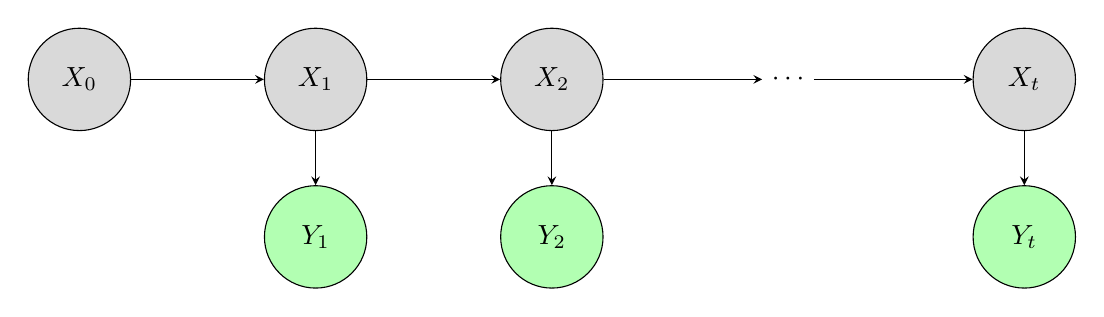
\begin{tikzpicture}[node distance=3cm, state/.style={circle, draw, minimum size=1.3cm, text centered}]
        
        % Nodos X y sus correspondientes Y con flechas entre ellos
        \node[state, fill=gray!30] (X0) {$X_{0}$};
        \node[state, fill=gray!30, right of=X0] (X1) {$X_{1}$};
        \node[state, fill=gray!30, right of=X1] (X2) {$X_{2}$};
        \node[right of=X2] (dots) {$\cdots$};
        \node[state, fill=gray!30, right of=dots] (Xt) {$X_{t}$};

        % Nodos Y correspondientes
        \node[state, fill=green!30, below of=X1, node distance=2cm] (Y1) {$Y_{1}$};
        \node[state, fill=green!30, below of=X2, node distance=2cm] (Y2) {$Y_{2}$};
        \node[state, fill=green!30, below of=Xt, node distance=2cm] (Yt) {$Y_{t}$};

        % Conexiones horizontales entre Xs con flechas
        \draw [-stealth] (X0) -- (X1);
        \draw [-stealth] (X1) -- (X2);
        \draw [-stealth] (X2) -- (dots);
        \draw [-stealth] (dots) -- (Xt);

        % Conexiones verticales entre X e Y correspondientes con flechas
        \draw [-stealth] (X1) -- (Y1);
        \draw [-stealth] (X2) -- (Y2);
        \draw [-stealth] (Xt) -- (Yt);

    \end{tikzpicture}
    \caption{Red bayesiana para el desarrollo de los PF}
    \label{fig:3.7}
\end{figure}


En la red bayesiana de la Figura \ref{fig:3.7} se declara que el valor de la variable oculta $X_{t}$ depende únicamente del valor de $X_{t-1}$, y que el valor de la variable observada $Y_{t}$ solamente depende de $X_{t}$. El comportamiento de cada problema se modela según la elección de las funciones $p\left(X_{t}|X_{t-1}\right)$ y $p\left(Y{t}|X{t}\right)$ para las dependencias anteriores. Sobre esta misma red se pueden definir varios problemas de estimación. En particular, para ejemplificar el funcionamiento se escogerá estimar $p\left(X_{0:t}|y_{1:t}\right)$ por medio de $p_{N}\left(X_{0:t}|y_{1:t}\right) = \displaystyle \sum_{i=1}^{N} w\left(x_{0:t}^{(i)}\right) \delta\left(X_{0:t} - x_{0:t}^{(i)}\right)$.

Este tipo de problemas se dan en diversas áreas del conocimiento: seguimiento de objetos, reconocimiento de habla, economía, etc \cite{pajares2010aprendizaje}. Un ejemplo del primer tipo es la determinación de la trayectoria $X_{0:t}$, seguida por una partícula móvil, a partir de las medidas $y_{1:t}$ captadas por uno o varios sensores.

\subsection{Filtros de partículas} \label{sec:Filtros de partículas}
El elemento principal de los PF es una implementación secuencial del método de muestreo enfatizado (\textit{Importance Sampling, IS}, \ref{subsec:IS}). Para aproximar $p\left(X_{0:t}|y_{1:t}\right)$ se usa una función de muestreo auxiliar $q\left(X_{0:t}|y_{1:t}\right)$, y se calcula el peso de $x_{0:t}^{(i)} \thicksim q\left(X_{0:t}|y_{1:t}\right)$ según la expresión $w\left(x_{0:t}^{(i)}\right) = \dfrac{p\left(x_{0:t}^{(i)}|y_{1:t}\right)}{q\left(x_{0:t}^{(i)}|y_{1:t}\right)}$. Utilizando el \textsl{teorema de Bayes}, la regla de la cadena y las relaciones de independencia condicional del problema, se manipulan las funciones de densidad para lograr la secuencialidad:

\begin{equation}
    \begin{aligned}
         p\left(X_{0:t}|y_{1:t}\right) &= p\left(X_{0:t},y_{1:t}\right)p\left(y_{1:t}\right) \quad \propto \\
         &\propto \quad p\left(y_{t}|X_{0:t},y_{1:t-1}\right)p\left(X_{t}|X_{0:t-1},y_{1:t-1}\right)p\left(X_{0:t-1},y_{1:t-1}\right) \\
         &= p\left(y_{t}|X_{t}\right)p\left(X_{t}|X_{t-1}\right)p\left(X_{0:t-1},y_{1:t-1}\right)p\left(y_{1:t-1}\right) \propto \\
         &\propto \quad p\left(y_{t}|X_{t}\right)p\left(X_{t}|X_{t-1}\right)p\left(X_{0:t-1},y_{1:t-1}\right)
    \end{aligned}
    \label{ec:3.9}
\end{equation}

\begin{equation}
    \begin{aligned}
        q\left(X_{0:t}|y_{1:t}\right) &= q\left(X_{t}|X_{0:t-1},y_{1:t}\right) q\left(X_{0:t-1}|y_{1:t}\right) \simeq \\
        &\simeq q\left(X_{t}|X_{0:t-1},y_{1:t}\right)q\left(X_{0:t-1}|y_{1:t-1}\right)
    \end{aligned}
    \label{ec:3.10}
\end{equation}

Sustituyendo en la expresión de los pesos, se ve qué pesos en tiempos consecutivos están relacionados, se obtiene una función auxiliar $q(\cdot)$ para el muestreo de $x_{t}^{(i)}$ y las funciones de densidad condicionales $p(\cdot)$ que definen el comportamiento dinámico del problema en su totalidad:

\begin{equation}
    \begin{aligned}
        w(x_{0:t}^{(i)}) &= \frac{p\left(x_{0:t}^{(i)}|y_{1:t}\right)}{q\left(x_{0:t}^{(i)}|y_{1:t}\right)} \simeq \frac{p\left(y_{t}|x_{t}^{(i)}\right)p\left(x_{t}^{(i)}|x_{t-1}^{(i)}\right)p\left(x_{0:t-1}^{(i)}|y_{1:t-1}\right)}{q\left(x_{t}^{(i)}|x_{0:t-1}^{(i)},y_{1:t}\right)q\left(x_{0:t-1}^{(i)},y_{1:t-1}\right)} = \\
        &= \frac{p\left(y_{t}|x_{t}^{(i)}\right)p\left(x_{t}^{(i)}|x_{t-1}^{(i)}\right)}{q\left(x_{t}^{(i)}|x_{0:t-1}^{(i)},y_{1:t}\right)}w\left(x_{0:t-1}^{(i)}\right)
    \end{aligned}
    \label{ec:3.11}
\end{equation}

Lo anteriormente expuesto se recoge en el pseudocódigo, mostrando el PF normalmente denominado \textit{Sequential
Importance Sampling, SIS}. La generación secuencial de las muestras, es decir, la obtención de $x_t^{(i)}$ correspondiente a la muestra $x_{0:t}^{(i)}$, es controlada por el bucle exterior de la Figura \ref{fig:3.8}, línea 1, mientras que los valores asociados a las $N$ muestras son controlados por el bucle interior. Las etapas opcionales muestran otras variantes, pero estos procesos no se realizan en el SIS.

Diferentes filtros de partículas tipo SIS surgen de la elección de distintas $q\left(X_{t}|X_{0:t-1},y_{1:t}\right)$. La elección óptima, sin tener en cuenta la función general $f\left(X_{0:t}\right)$, es $q^*\left(X_{t}|X_{0:t-1},y_{1:t}\right) = p\left(X_t|X_{t-1},y_t\right)$ \cite{pajares2010aprendizaje}. Por lo general, no es posible generar muestras a partir de la misma, por lo que lo más sencillo es elegir $q\left(X_{t}|X_{0:t-1},y_{1:t}\right) = p\left(X_t|x_{t-1}^{(i)}\right)$, que figura en las primeras versiones de los PF tipo SIS, útil porque facilita la generación de muestras y los cálculos de los pesos $w\left(x_{0:t}^{(i)}\right) = p\left(y_t|x_t^{(i)}\right)w\left(x_{0:t-1}^{(i)}\right)$.

Sin embargo, una elección distinta a la óptima hace que con el tiempo el número de muestras que toman un valor de peso nulo se incremente, provocando una degeneración de las muestras. Al no contribuir al cálculo integral, hace menos eficiente el algoritmo, por lo que se requiere de otras técnicas para compensarlo: se combina el SIS con etapas de remuestreo por pesos (\textit{Weighted Resampling, WR}, \ref{subsec:WR}).

\begin{figure}[ht]
    \centering
    \begin{tcolorbox}[colframe=black, colback=white, boxrule=0.5pt, width=0.87\textwidth, sharp corners]
        \parbox[t]{0.1\linewidth}{1.} \parbox[t]{0.85\linewidth}{for $(i=1:N)$} \\[0.5em]
        \parbox[t]{0.1\linewidth}{2.} \parbox[t]{0.85\linewidth}{\hspace{1em}set $x_0^{(i)}, \quad \text{set } w\left(x_0^{(i)}\right)$} \\[0.5em]
        \parbox[t]{0.1\linewidth}{3.} \parbox[t]{0.85\linewidth}{$t = 1$} \\[0.5em]
        \parbox[t]{0.1\linewidth}{4.} \parbox[t]{0.85\linewidth}{while (true)} \\[0.5em]
        \parbox[t]{0.1\linewidth}{5.} \parbox[t]{0.85\linewidth}{\hspace{1em} $F=0$} \\[0.5em]
        \parbox[t]{0.1\linewidth}{6.} \parbox[t]{0.85\linewidth}{\hspace{1em} optionally, WR for Auxiliary PF} \\[0.5em]
        \parbox[t]{0.1\linewidth}{7.} \parbox[t]{0.85\linewidth}{\hspace{1em} for $(i=1:N)$} \\[0.5em]
        \parbox[t]{0.1\linewidth}{8.} \parbox[t]{0.85\linewidth}{\hspace{2em} $x_t^{(i)} \sim q\left(X_{t}|X_{0:t-1},y_{1:t}\right), \quad \dfrac{p\left(y_{t}|x_{t}^{(i)}\right)p\left(x_{t}^{(i)}|x_{t-1}^{(i)}\right)}{q\left(x_{t}^{(i)}|x_{0:t-1}^{(i)},y_{1:t}\right)}w\left(x_{0:t-1}^{(i)}\right)$} \\[0.5em]
        \parbox[t]{0.1\linewidth}{9.} \parbox[t]{0.85\linewidth}{\hspace{2em} $F = F+w\left(x_{0:t}^{(i)}\right)$} \\[0.5em]
        \parbox[t]{0.1\linewidth}{10.} \parbox[t]{0.85\linewidth}{\hspace{1em} for $(i=1:N)$} \\[0.5em]
        \parbox[t]{0.1\linewidth}{11.} \parbox[t]{0.85\linewidth}{\hspace{2em} $w\left(x_{0:t}^{(i)}\right) = \dfrac{w\left(x_{0:t}^{(i)}\right)}{F}$} \\[0.5em]
        \parbox[t]{0.1\linewidth}{12.} \parbox[t]{0.85\linewidth}{\hspace{1em} \textsl{optionally}, WR por SIR} \\[0.5em]
        \parbox[t]{0.1\linewidth}{13.} \parbox[t]{0.85\linewidth}{\hspace{1em} $t=t+1$}
    \end{tcolorbox}
    \caption{Filtro de partículas Sequential Importance Sampling (SIS) con las
etapas opcionales que lo convierten en Sequential Importance Resampling (SIR) y
Auxiliary Particle Filter (APF).}
    \label{fig:3.8}
\end{figure}

Sobre el pseudocódigo de la Figura \ref{fig:3.8}, en la etapa asociada a la parte \textit{optionally, WR for SIR}, utiliza $r\left(x_{0:t}^{(i)}\right) = w\left(x_{0:t}^{(i)}\right)$. En esta modalidad del filtro de partículas \textit{Sampling Importance Resampling, SIR}, los pesos de las muestras tras el remuestreo son $w\left(x_{0:t}^{(i)}\right) = \dfrac{1}{N}$, y las muestras $x_{0:t}^{(i)}$ se acumulan en regiones donde previamente los pesos toman valores no nulos.
El problema que surge de aplicar esto, indiscriminadamente, es el contrario al anterior, el empobrecimiento. Ahora, la variable $X_k$ tiende a tomar el mismo valor en todas las muestras $x_{0:t}^{(i)}$, para algún $k < t$. Para evitarlo, puede aplicarse solamente a las iteraciones $t$ en las que se detecte la degeneración mediante algún proceso auxiliar como el cálculo del número efectivo de partículas.

Además, en la parte del pseudocódigo \textit{optionally, WR for Auxiliary PF}, se utiliza $r\left(x_{0:t-1}^{(i)}\right) = p\left(y_t|x_{0:t-1}^{(i)}\right)$, haciendo que el remuestreo considere las dependencias entre la nueva medida y los valores disponibles de la muestra. Calcular el valor de la función no es, en la mayoría de los casos, sencillo, de modo que se usa la aproximación \ref{ec:3.12}.

Esta etapa, WR, junto a la función de muestreo $q\left(X_{t}|X_{0:t-1},y_{1:t}\right) = p\left(X_t|x_{t-1}^{(i)}\right)$, se utilizan de manera auxiliar en el conocido como \textit{Auxiliary PF (APF)}, por lo que los pesos de las partículas al finalizar cada iteración son $w\left(x_{0:t}^{(i)}\right) \propto p\left(y_t|x_t^{(i)}\right)/ p\left(y_t|m_t^{(i)}\right)$:

\begin{equation}
    \begin{aligned}
        &p\left(y_t|x_{0:t-1}^{(i)}\right) = \int p\left(y_t|X_t\right)p\left(X_t|x_{t-1}^{(i)}\right)dX_t \simeq \\
        &\simeq p\left(y_t|m_t^{(i)}\right)p\left(X_t|x_{t-1}^{(i)}\right)dX_t = p\left(y_t|m_t^{(i)}\right) ; \quad \text{con} \quad m_t^{(i)} = E_{p\left(X_t|x_{t-1}^{(i)}\right)}[X_t]
    \end{aligned}
    \label{ec:3.12}
\end{equation}

Todas las combinaciones vistas de $q\left(X_{t}|X_{0:t-1},y_{1:t}\right)$ y etapas de WR generan distintos algoritmos secuenciales de simulación, con el objetivo final de generar las muestras en las zonas importantes del espacio, por lo que cualquier conocimiento previo que pueda facilitar la generación de las muestras en las regiones de interés puede ser una guía para la elección de $q\left(X_{t}|X_{0:t-1},y_{1:t}\right)$ y de las funciones $r\left(X_{0:t}\right)$ para las etapas de WR.

\section{Métodos de simulación generales}
Los métodos introducidos hasta ahora, (RS, IS, WR, MC), pueden ser caracterizados por aproximar una función de densidad original $p\left(\cjtoVarAl\right)$ mediante una auxiliar $p_N\left(\cjtoVarAl\right)$ comprendida por múltiples $p\left(\cjtoVarAl - \unCjtoVarAli\right)$, obtenidas a partir de un muestreo realizado con las funciones de muestreo auxiliar $q(\cdot)$, y ponderadas por medio de $w\left(\unCjtoVarAli\right)$. Sin embargo, se pueden destacar importantes discrepancias entre ellos:
\begin{enumerate}
    \item Tipo de $p\left(\cjtoVarAl\right)$: para WR está compuesta por varias funciones de densidad puntual, mientras que en el resto es una densidad genérica.
    \item Función de muestreo auxiliar $q(\cdot)$:
    \begin{enumerate}
        \item RS genera las muestras $\unCjtoVarAli$ según una función genérica $q\left(\cjtoVarAl\right)$, y decide su aceptación o rechazo en función de la discrepancia entre $p\left(\unCjtoVarAli\right)$ y $q\left(\unCjtoVarAli\right)$, por lo que su eficiencia la marca la cantidad de valores rechazados.
        \item IS muestrea las $\unCjtoVarAli$ por medio de $q\left(\cjtoVarAl\right)$, pero asigna un peso $w\left(\unCjtoVarAli\right)$ proporcional a la discrepancia anterior.
        \item WR se asemeja a IS, solo que utiliza una función muestreo proporcional a una redistribución de las muestras según $r\left(\unCjtoVarAli\right)$.
        \item MC genera las muestras siguiendo la cadena $K\left(\cjtoVarAl|\unCjtoVarAliMenos\right)$, con ciertas propiedades, rechazando las muestras anteriores a la convergencia.
    \end{enumerate}
    \item Los pesos $w\left(\unCjtoVarAli\right)$ asociados a las funciones de densidad puntual $p\left(\cjtoVarAl-\unCjtoVarAli\right)$: en RS y MC todas las muestras tienen la misma importancia $\left(w\left(\unCjtoVarAli\right) = N^{-1}\right)$, mientras que en IS y WR, los pesos dependen de la función de distribución elegida. Por eso, en unos se ignora y en otros se trabaja con el par muestra-peso
    \item Si el método funciona cuando desconocemos la expresión de $p\left(\cjtoVarAl\right)$ pero se dispone de $Cte\cdot p\left(\cjtoVarAl\right)$: aplica a RS, IS, WR, pero no a MC, sus cadenas no necesariamente tienen por qué funcionar con ese múltiplo de la función de densidad.
\end{enumerate}

Adicionalmente, también se debe tener en cuenta la paralización de cada uno de los cuatro métodos, pues no todos generan las muestras a la misma velocidad.
En IS y WR, el valor de las muestras y de los pesos sin normalizar se realiza de forma independiente, de modo que puede hacerse de manera simultánea. RS funciona de manera similar, pues el valor de cada muestra y su aceptación o rechazo se realiza de forma independiente, salvo que discrepa en la cantidad de muestras generadas, ya que depende de cuántas haya rechazado, hasta llegar a $N$. Finalmente, se recuerda que en MC las cadenas generan valores para la muestra de manera condicionada al anterior valor, $K\left(\cjtoVarAl|\unCjtoVarAliMenos\right)$, de modo que es necesario hacerlo de manera secuencial. Por otro lado, también es posible generar de forma simultánea varios conjuntos de muestras mediante varias cadenas de Markov ejecutadas en paralelo, de forma independiente.

Se recuerda también que en IS la función óptima de muestreo es proporcional a $\abs{f\left(\cjtoVarAl\right)}$, por lo que es inútil generar puntos en regiones donde dicha función sea nula. Esto se puede extender al resto de métodos, pues tales puntos no aportan valor a la aproximación integral.

Para finalizar, se contrastan los métodos RS frente a una combinación de una etapa de IS con una de WR, donde $r\left(\unCjtoVarAli\right)$ sean idénticas a los de la función original $\sum \alpha^{(i)}\delta\left(\cjtoVarAl-\unCjtoVarAli\right)$.
En RS, la generación de las posibles muestras $\unCjtoVarAli$ generadas con $q\left(\cjtoVarAl\right)$ se da en la etapa de muestreo de IS con $q\left(\cjtoVarAl\right)$.
Los pesos $\unPeso = \dfrac{p\left(\unCjtoVarAli\right)}{q\left(\unCjtoVarAli\right)}$ en IS para las muestras son proporcionales a Pr$\left(A|\unCjtoVarAli\right)=\dfrac{p\left(\unCjtoVarAli\right)}{Mq\left(\unCjtoVarAli\right)}$ en el proceso de aceptación/rechazo para cada una de las muestras de RS.
En la última etapa, mientras que RS hace el proceso de aceptación/rechazo de la muestra de forma independiente a las demás, el uso de una etapa de WR tras una de IS con $r\left(\unCjtoVarAli\right)=\dfrac{p\left(\unCjtoVarAli\right)}{q\left(\unCjtoVarAli\right)}$ hace que las muestras admitidas (y posiblemente repetidas) sean aquellas con valores $\dfrac{r(\unCjtoVarAli)}{\displaystyle \sum r(\unCjtoVarAli)}$ más significativos. Tras la etapa de WR, los pesos de las $N$ muestras son equiponderantes, y el mismo valor se les asigna tras la etapa de RS.

Ambos métodos se comportan de forma parecida para $N\rightarrow\infty$ debido a que, en RS, sólo se usa un valor $M$ a lo largo de todo el soporte de $p(\cjtoVarAl)$, al igual que su análogo $\displaystyle \sum_{i=1}^N r(\unCjtoVarAli)$ en WR.


